\documentclass[a4paper,14pt]{extarticle}

\usepackage[a4paper,top=20mm,bottom=20mm,left=30mm,right=10mm]{geometry}
\usepackage[T1,T2A]{fontenc}
\usepackage[utf8]{inputenc}
\usepackage[russian]{babel}
\usepackage{indentfirst}
\usepackage{titlesec}
\usepackage{graphicx}
\usepackage{verbatim}
\usepackage{fancyvrb}

\renewcommand{\baselinestretch}{1.3}
\titleformat{\section}{\normalsize\bfseries}{\thesection}{1em}{}
\titleformat{\subsection}{\normalsize\bfseries}{\thesection}{1em}{}
\setlength{\parindent}{12.5mm}

\begin{document}

  \newpage\thispagestyle{empty}
  \begin{center}
    \MakeUppercase{
      Министерство науки и высшего образования Российской Федерации\\
      Федеральное государственное бюджетное образовательное учреждение высшего образования\\
      <<Вятский Государственный Университет>>\\
    }
    Институт математики и информационных систем\\
    Факультет автоматики и вычислительной техники\\
    Кафедра электронных вычислительных машин
  \end{center}
  \vfill

  \begin{center}
    Отчет по лабораторной работе №2.1\\
    по дисциплине\\
    <<Управление данными>>\\
    «Основы DML-запросов в PostgreSQL»\\
  \end{center}
  \vfill

  \noindent
  \begin{tabular}{ll}
    Выполнил студент гр. ИВТб-2301-05-00 \hspace{5mm} &
    \rule[-1mm]{25mm}{0.10mm}\,/Макаров С.А./\\
    
    Преподаватель & \rule[-1mm]{25mm}{0.10mm}\,/Клюкин В.Л./\\
  \end{tabular}

  \vfill
  \begin{center}
    Киров 2025
  \end{center}

  \newpage
  \section*{Цель}
  Цель лабораторной работы: освоить основные варианты DML-запросов в PostgreSQL, научиться создавать SQL-скрипты для заполнения таблиц данными, познакомиться с типами данных в PostgreSQL, освоить основные варианты DDL-запросов в PostgreSQL, научиться использованию команды update и delete, научиться работать с представлениями.

  \section*{Задание}
  \begin{enumerate}
    \item Создать и выполнить SQL-скрипт, который будет заполнять таблицы данными. Нужно добавить не менее 3-5 строк в каждую таблицу.
    \item Создать представления для нескольких таблиц, в которых собираются данные из самой таблицы и других, на которые она ссылается. Выборка из любого представления должна давать полную и осмысленную информацию по сущностям. Хотя бы одно из представлений должно быть сделано с использованием соединений (join) в запросе
  \end{enumerate}

  \pagebreak
  \section*{Решение}
  Ниже представлен скрипт, выполняющий заполнение базы данных в таблицы с информацией о пользователях, способах оплаты, категориях продуктов, продуктах, ингредиентах, вариантах продукта.

  \noindent
  \begin{Verbatim}[tabsize=4,fontsize=\small]
DO $$
DECLARE

userId BIGINT;
paymentId BIGINT;
categoryId BIGINT;
productId BIGINT;
ingredientId BIGINT;

BEGIN

INSERT INTO "users"(phone_number, username)
VALUES ('89000000000', 'Николай')
RETURNING id INTO userId;

INSERT INTO "payments" (title)
VALUES ('Мир')
RETURNING id INTO paymentId;

INSERT INTO "user_payments" (user_id, payment_id, card_number, cvv)
VALUES (userId, paymentId, '2400100020003000', '135');

INSERT INTO "payments" (title)
VALUES ('Visa')
RETURNING id INTO paymentId;

INSERT INTO "user_payments" (user_id, payment_id, card_number, cvv)
VALUES (userId, paymentId, '6500100020003000', '246');

INSERT INTO "users" (phone_number, username)
VALUES ('89001110000', 'Александр')
RETURNING id INTO userId;

INSERT INTO "user_payments" (user_id, payment_id, card_number, cvv)
VALUES (userId, paymentId, '6500300020001000', '975');

INSERT INTO "users" (phone_number, username)
VALUES ('89002220000', 'Екатерина')
RETURNING id INTO userId;

INSERT INTO "payments" (title)
VALUES ('MasterCard')
RETURNING id INTO paymentId;

INSERT INTO "user_payments" (user_id, payment_id, card_number, cvv)
VALUES (userId, paymentId, '4200400050006000', '864');

INSERT INTO "categories" (title)
VALUES ('Пиццы')
RETURNING id INTO categoryId;

INSERT INTO "products" (category_id, title)
VALUES (categoryId, 'Карбонара')
RETURNING id INTO productId;

INSERT INTO "ingredients" (title, image_url, price)
VALUES ('Сырный бортик', 'https://cdn.dodostatic.net/static
              /Img/Ingredients/99f5cb91225b4875bd06a26d2e842106.png', 179)
RETURNING id INTO ingredientId;

INSERT INTO "product_ingredients" (product_id, ingredient_id, is_required)
VALUES (productId, ingredientId, TRUE)
RETURNING id INTO ingredientId;

INSERT INTO "ingredients" (title, image_url, price)
VALUES ('Пряная говядина', 'https://cdn.dodostatic.net/static
              /Img/Ingredients/11ef5ed5f8f64595a6d6a99c1fe6f7f0.png', 119)
RETURNING id INTO ingredientId;

INSERT INTO "product_ingredients" (product_id, ingredient_id, is_required)
VALUES (productId, ingredientId, TRUE)
RETURNING id INTO ingredientId;

INSERT INTO "ingredients" (title, image_url, price)
VALUES ('Моцарелла', 'https://cdn.dodostatic.net/static
              /Img/Ingredients/cdea869ef287426386ed634e6099a5ba.png', 79)
RETURNING id INTO ingredientId;

INSERT INTO "product_ingredients" (product_id, ingredient_id, is_required)
VALUES (productId, ingredientId, TRUE)
RETURNING id INTO ingredientId;

INSERT INTO "ingredients" (title, image_url, price)
VALUES ('Свежие томаты', 'https://cdn.dodostatic.net/static
              /Img/Ingredients/000D3A39D824A82E11E9AFA7AC1A1D67', 59)
RETURNING id INTO ingredientId;

INSERT INTO "product_ingredients" (product_id, ingredient_id, is_required)
VALUES (productId, ingredientId, DEFAULT)
RETURNING id INTO ingredientId;

INSERT INTO "ingredients" (title, image_url, price)
VALUES ('Сладкий перец', 'https://cdn.dodostatic.net/static
              /Img/Ingredients/000D3A22FA54A81411E9AFA63F774C1B', 59)
RETURNING id INTO ingredientId;

INSERT INTO "product_ingredients" (product_id, ingredient_id, is_required)
VALUES (productId, ingredientId, DEFAULT)
RETURNING id INTO ingredientId;

INSERT INTO "product_variants" (product_id, image_url, size, weight, price)
VALUES (productId, 'https://media.dodostatic.net/image/r:292x292/
                    0196361c3c34728dbed2f01a37f04284.jpg', 20, 220, 479);

INSERT INTO "product_variants" (product_id, image_url, size, weight, price)
VALUES (productId, 'https://media.dodostatic.net/image/r:292x292/
                    019591b1343c746bb4c108bede4d469c.jpg', 25, 410, 659);

INSERT INTO "product_variants" (product_id, image_url, size, weight, price)
VALUES (productId, 'https://media.dodostatic.net/image/r:292x292/
                    019591b13a1a724b90092c16d9b1c05a.jpg', 30, 590, 1009);
INSERT INTO "product_variants" (product_id, image_url, size, weight, price)
VALUES (productId, 'https://media.dodostatic.net/image/r:292x292/
                    019591b14a2e7663a8daf17169cfd23f.jpg', 35, 800, 1119);

INSERT INTO "categories" (title)
VALUES ('Закуски')
RETURNING id INTO categoryId;

INSERT INTO "products" (category_id, title, description)
VALUES (categoryId, 'Додстер', 'Легендарная горячая закуска с цыпленком, 
              томатами, моцареллой, соусом ранч в тонкой пшеничной лепешке')
RETURNING id INTO productId;

INSERT INTO "product_variants" (product_id, image_url, weight, price)
VALUES (productId, 'https://media.dodostatic.net/image/r:292x292/
                    01980cb92528769295aeb186fb501f8e.jpg', 190, 249);

INSERT INTO "categories" (title)
VALUES ('Завтрак')
RETURNING id INTO categoryId;

INSERT INTO "products" (category_id, title, description)
VALUES (categoryId, 'Омлет с ветчиной и грибами в пите', 'Горячий сытный омлет 
    с поджаристой корочкой, ветчина, шампиньоны и моцарелла в пшеничной пите. 
    Удобно взять с собой')
RETURNING id INTO productId;

INSERT INTO "product_variants" (product_id, image_url, weight, price)
VALUES (productId, 'https://media.dodostatic.net/image/r:292x292/
                    019860510daa726fa023e04a1ae06a87.jpg', 170, 239);

INSERT INTO "categories" (title)
VALUES ('Десерты')
RETURNING id INTO categoryId;

INSERT INTO "products" (category_id, title, description)
VALUES (categoryId, 'Чизкейк Банановый с шоколадным печеньем', 
        'Солнечная версия классического рецепта: нежный чизкейк 
        с бананом и шоколадным печеньем')
RETURNING id INTO productId;

INSERT INTO "product_variants" (product_id, image_url, weight, price)
VALUES (productId, 'https://media.dodostatic.net/image/r:292x292/
                    0198138723e478fba518947539dbbdcb.jpg', 100, 189);

INSERT INTO "categories" (title)
VALUES ('Коктейли')
RETURNING id INTO categoryId;

INSERT INTO "products" (category_id, title, description)
VALUES (categoryId, 'Молочный коктейль Фисташка', 'Сочетание нежности, 
                        сливочной текстуры и тонкого вкуса фисташки')
RETURNING id INTO productId;

INSERT INTO "product_variants" (product_id, image_url, weight, volume, price)
VALUES (productId, 'https://media.dodostatic.net/image/r:292x292/
                    0198138723e478fba518947539dbbdcb.jpg', 320, 300, 269);

INSERT INTO "product_variants" (product_id, image_url, weight, volume, price)
VALUES (productId, 'https://media.dodostatic.net/image/r:292x292/
                    0198138723e478fba518947539dbbdcb.jpg', 500, 400, 439);

INSERT INTO "categories" (title)
VALUES ('Кофе')
RETURNING id INTO categoryId;

INSERT INTO "products" (category_id, title, description)
VALUES (categoryId, 'Кофе Капучино', 'Легендарный рецепт кофе: 
                  эспрессо, горячее молоко и плотная молочная пенка')
RETURNING id INTO productId;

INSERT INTO "product_variants" (product_id, image_url, weight, volume, price)
VALUES (productId, 'https://media.dodostatic.net/image/r:292x292/
                    019840b6488170018dd640026aea9961.jpg', 240, 400, 179);

end;
$$ language plpgsql;
  \end{Verbatim}

  Создадим представление, которое будет отображать все способы оплаты пользователей. Представление содержит номер телефона пользователя, имя пользователя, номер банковской карты, CVV код, тип банковской карты. Результат выборки представлен на рисунке 1. Соотвествующий SQL-скрипт представлен ниже:

    \noindent
  \begin{Verbatim}[tabsize=4,fontsize=\small]
CREATE OR REPLACE VIEW "users_payments_v" AS
SELECT u.phone_number AS "Номер телефона", u.username AS "Имя пользователя", 
up.card_number AS "Номер карты", up.cvv AS "CVV код", p.title AS "Тип карты"
FROM "users" u
  JOIN "user_payments" up on u.id = up.user_id
  JOIN "payments" p on p.id = up.payment_id;

SELECT * FROM "users_payments_v";
  \end{Verbatim}

  \begin{figure}[h]
    \centering
    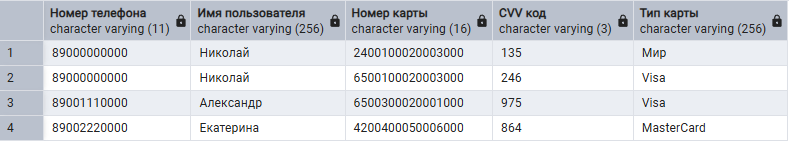
\includegraphics[width=1\linewidth]{img/view-1}
  \end{figure}
  \begin{center}
    Рисунок 1 – Результат выборки представления
  \end{center}

  Создадим представление, которое будет отображать все категории и продукты, принадлежащие им. Представление содержит название категории, название продукта, описание продукта. Результат выборки представлен на рисунке 2. Соотвествующий SQL-скрипт представлен ниже:

  \noindent
  \begin{Verbatim}[tabsize=4,fontsize=\small]
CREATE OR REPLACE VIEW "categories_products_v" AS
SELECT c.title AS "Категория", p.title AS "Название продукта", 
p.description AS "Описание продукта"
FROM "categories" c
  JOIN "products" p on c.id = p.category_id;

SELECT * FROM "categories_products_v";
  \end{Verbatim}

  \begin{figure}[h]
    \centering
    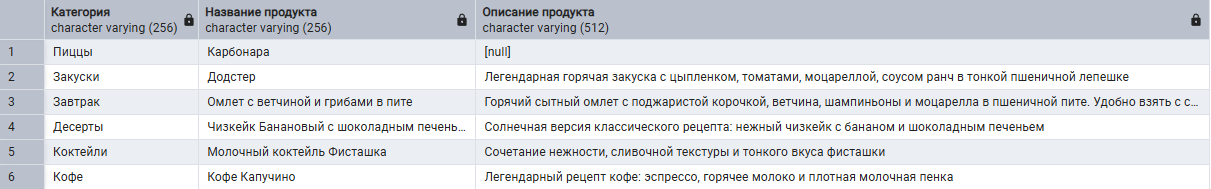
\includegraphics[width=1\linewidth]{img/view-2}
  \end{figure}
  \begin{center}
    Рисунок 2 – Результат выборки представления
  \end{center}

  Создадим представление, которое будет отображать все обязательные ингредиенты продукта. Представление содержит название продукта, ингредиент, цену ингредиента. Результат выборки представлен на рисунке 3. Соотвествующий SQL-скрипт представлен ниже:

  \noindent
  \begin{Verbatim}[tabsize=4,fontsize=\small]
CREATE OR REPLACE VIEW "products_required_ingredients_v" AS
SELECT p.title AS "Название продукта", i.title AS "Ингредиент", 
i.price AS "Цена ингредиента" 
FROM "products" p
  JOIN "product_ingredients" pi on p.id = pi.product_id
  JOIN "ingredients" i on i.id = pi.ingredient_id
WHERE pi.is_required = true;

SELECT * FROM "products_required_ingredients_v";
  \end{Verbatim}

  \begin{figure}[h]
    \centering
    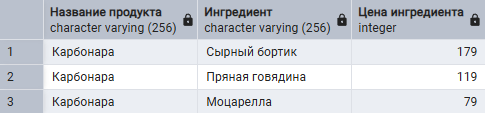
\includegraphics[width=0.75\linewidth]{img/view-3}
  \end{figure}
  \begin{center}
    Рисунок 3 – Результат выборки представления
  \end{center}

  \section*{Вывод}
  В ходе выполнения лабораторной работы изучены основы DML - запросов в PostgreSQL, такие как запросы на вставку данных, запросы на выборку и создание представлений. Исходя из вышеописанного созданы запросы на вставку данных, созданы представления с выборкой данных с соединениями с другими таблицами.

\end{document}